\documentclass[12pt,a4paper]{article}

    \usepackage[margin=1.2in]{geometry}
    \usepackage{caption}
    \usepackage{graphicx}
    \usepackage{subcaption}
    %\usepackage{mwe}
    
    
    %opening
    \title{\huge{Structural Reconstruction of a Ruined Building}\\ \vspace{1cm}\large{CS5240 - Theoretical Foundations in Multimedia}\\
        \large{Project Group : P-03}}
    
    
    \date{}
    
    
    %\author{Anshul Aggarwal\\A0191501R \and Gogula Krishnan Saravanan\\A0191385X \and Manasa Kashyap\\A0178462W \and Meenakshi Sundaram Viswanathan\\A0191324L}
    
    
    \begin{document}
    
    \maketitle
    \vspace{-1.6cm}
    \begin{table}[h]
        \centering
        \begin{tabular}{cc}
            \textbf{\large{Anshul Aggarwal}} & \textbf{\large{Gogula Krishnan Saravanan}}      \vspace{0.2cm}\\
            A0191501R                & A0191385X                               \vspace{0.5cm}\\
            \textbf{\large{Manasa Kashyap}}  & \textbf{\large{Meenakshi Sundaram Viswanathan}} \vspace{0.2cm}\\
            A0178462W                & A0191324L                              
        \end{tabular}
    \end{table}
    
    %\begin{abstract}
    
    %\end{abstract}
    
    \section{Introduction}
    
    Ruined buildings, or simply ruins, are the remains of the man-made buildings. Over the passage of time, due to various reasons such as natural disaster, deliberate acts of destruction, or simply weathering and lack of maintenance, only parts of the original building remain today.
    
    There are various scenarios where reconstructed models of these ruined buildings may be useful. Archaeologists and historians refer to ruins of ancient buildings (like the one shown in Fig. \ref{fig:ruins}) to study civilizations, their style of architecture, and their culture. A fully reconstructed model may help them study the structure better. Other than that, engineers need to fix damages to buildings caused by natural disasters or explosions, and such a reconstructed model will help them plan out repairs.
    
    Our work here aims to efficiently employ data fitting/model fitting techniques to reconstruct the defining structures of any dilapidated building, so as to achieve a structure that closely resembles the original structural design of the building under consideration.
    
    \begin{figure}
        \centering
        \captionsetup{justification=centering}
        
        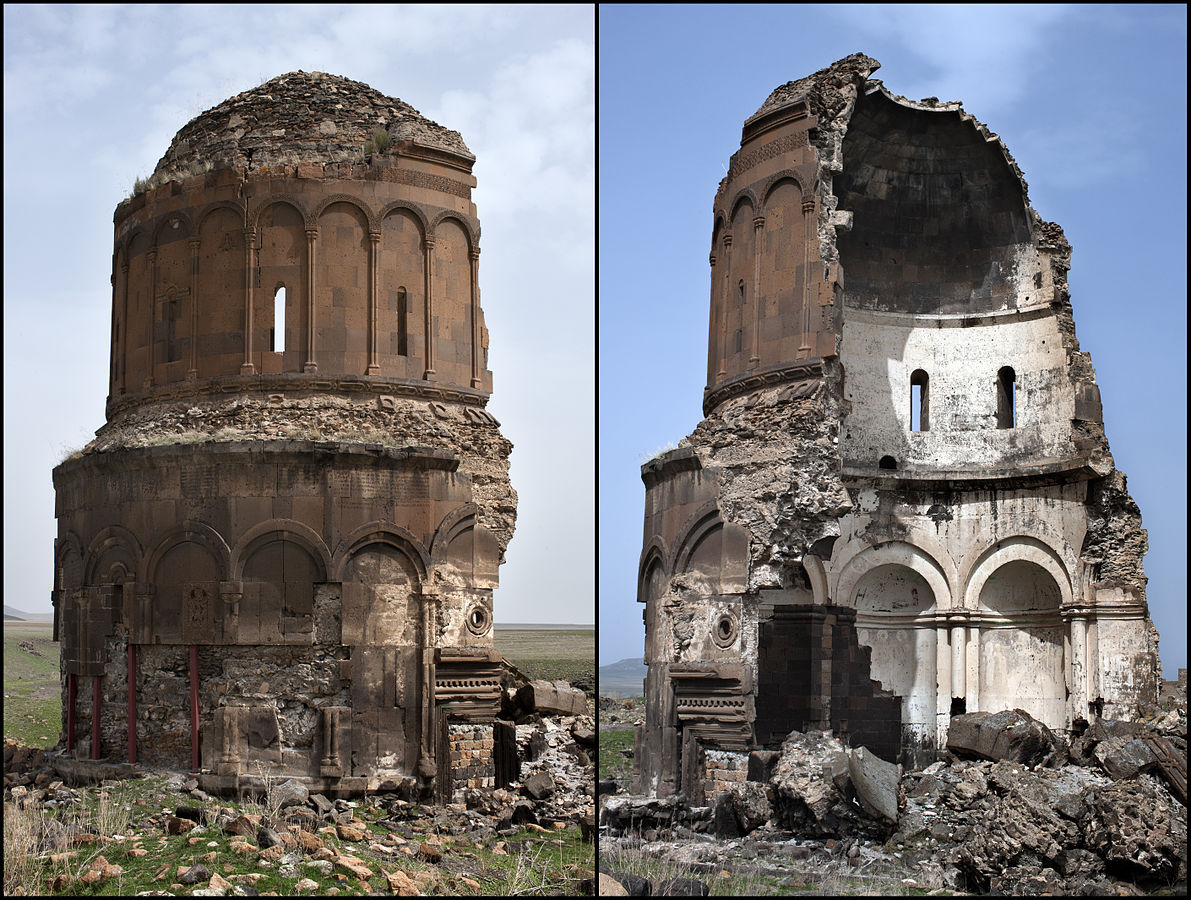
\includegraphics[width=0.8\textwidth]{ruins.jpg}
        
        \caption{The Church of the Holy Redeemer -- Ani, Turkey}
        \label{fig:ruins}
    \end{figure}
    
    \section{Variables and Relationships}
    
    A 3-dimensional point cloud of the existing structure will act as the input to our problem. These points may have been captured using 3D Laser Scanning, or obtained by any other means.
    
    We try to reconstruct surfaces from these points by defining relationships, or functions over the 3D space which are satisfied by the input points, such that they best represent the original shape of the building. These surfaces may represent walls, ceilings, floors, or any other surfaces.
    
    \section{Problem Definition}
    
    \subsection{Objective}
    
    Given a point cloud representation of a ruined building, obtain surface functions of the building to recreate a model of the building that could best represent it before it was damaged.
    
    \subsection{Input}
    
    \begin{itemize}
        \item $n$ data points capturing external structure of ruined building with 3D coordinates $p_i = [x_i, y_i, z_i]^\top, i = 1,\dots,n$
    \end{itemize}
    
    \subsection{Outputs}
    
    \begin{itemize}
        \item Number of surfaces: $k$.
        \item $k$ surface functions $f_j, j=1,\dots,k$, constrained by boundary conditions.
    \end{itemize}
    
    \subsection{Constraints}
    For all points $p_i = [x_i,y_i,z_i]^\top$, $p_i \in S_j \subset \{p_1,\dots,p_n\} $ satisfying the following boundary limits for the $j^{th}$ surface.
    
    \indent $a1_j<x_i<b1_j$ where $a1_j,b1_j \in \mathbf{R}$
    
    \indent $a2_j<y_i<b2_j$ where $a2_j,b2_j \in \mathbf{R}$
    
    \indent $a3_j<z_i<b3_j$ where $a3_j,b3_j \in \mathbf{R}$
    
    \noindent The spatial error $E_j$ is minimized for each surface $f_j, j=1,\dots,k$ for all points in $S_j $.
    
    \begin{equation}
    \textrm{Minimize } E_j = \sum_{p_i \in S_j} {||f_j(p_i) - p_i ||^2} %Standard minimization notation, and makes single glance read easier to understand%
    \end{equation}
    
    \section{Observations \& Issues}\label{issues}
    
    There may be instances where some information about the building structure is completely lost. This lost information cannot be regained. For example, if an asymmetric or non-uniform corner of a building is completely lost, the reconstruction may not be able to accurately reflect the original building, as there is no information to define the asymmetry.
    
    An extension of this problem is when information about a dimension of the building is lost. This may lead to multiple output reconstructed models based on different guesses for the missing dimension.
    
    \section{Problem Instance and Expected Results}
    
    Let us consider an example. Fig. \ref{fig:scatter} shows the point cloud of a dilapidated, ruined building. To an observer, there may be a few obvious missing parts of the building, or regions in the 3D space where the point density is high in the neighbourhood, while zero in the given region. This is represented in Fig. \ref{fig:missing}.
    
    This is however difficult to recreate in computational terms. We therefore use data fitting to obtain surfaces that best fit the given data points, and considering these surfaces shall intersect to define boundaries, we can get the missing or damaged portions of the building. There may however be multiple possible reconstructions, as discussed in section \ref{issues} above. Considering two different reconstruction scenarios, we may get two distinct models, as shown in Fig. \ref{fig:rec1}, \ref{fig:rec2}. These reconstructed models however only differ mostly in the intersection based bounds for the fitted surfaces, and not the surfaces themselves.
    
    \begin{figure*}
        \centering
        \begin{subfigure}[b]{0.475\textwidth}
            \centering
            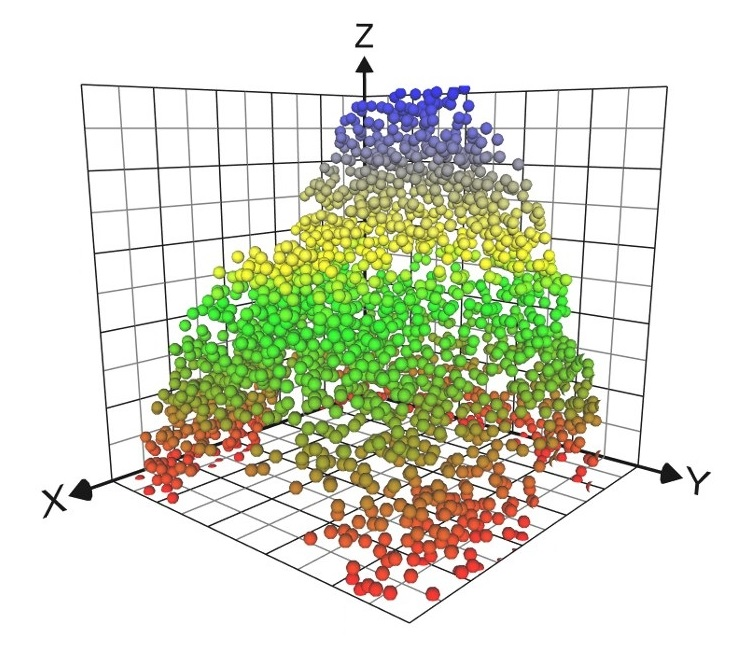
\includegraphics[width=\textwidth]{scatter1.jpg}
            \caption[]{{\small Point cloud representation of a ruined building}}    
            \label{fig:scatter}
        \end{subfigure}
        \hfill
        \begin{subfigure}[b]{0.475\textwidth}  
            \centering 
            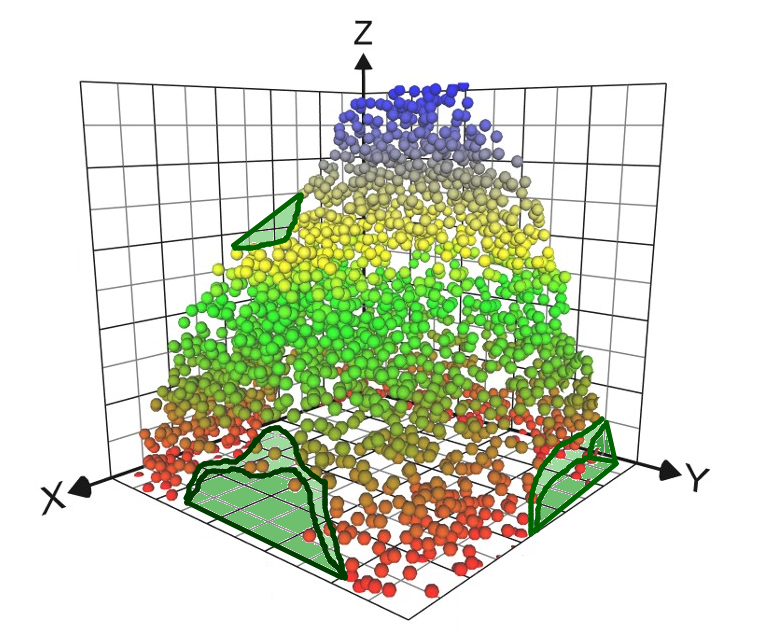
\includegraphics[width=\textwidth]{missing2.png}
            \caption[]{{\small Missing or damaged parts of the building}}    
            \label{fig:missing}
        \end{subfigure}
        \vskip\baselineskip
        \begin{subfigure}[b]{0.475\textwidth}   
            \centering 
            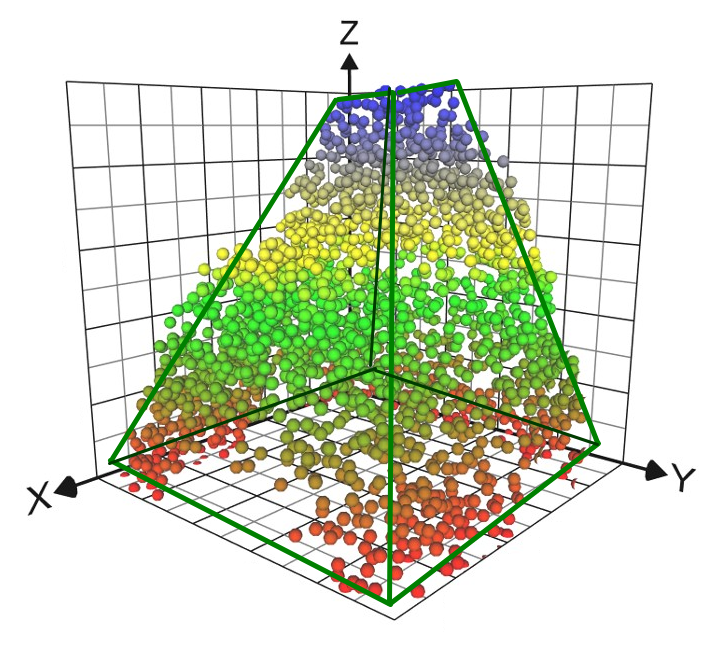
\includegraphics[width=\textwidth]{reconstruction.png}
            \caption[]{{\small Reconstruction scenario 1 - levelling of the planes at the top}}    
            \label{fig:rec1}
        \end{subfigure}
        \quad
        \begin{subfigure}[b]{0.475\textwidth}   
            \centering 
            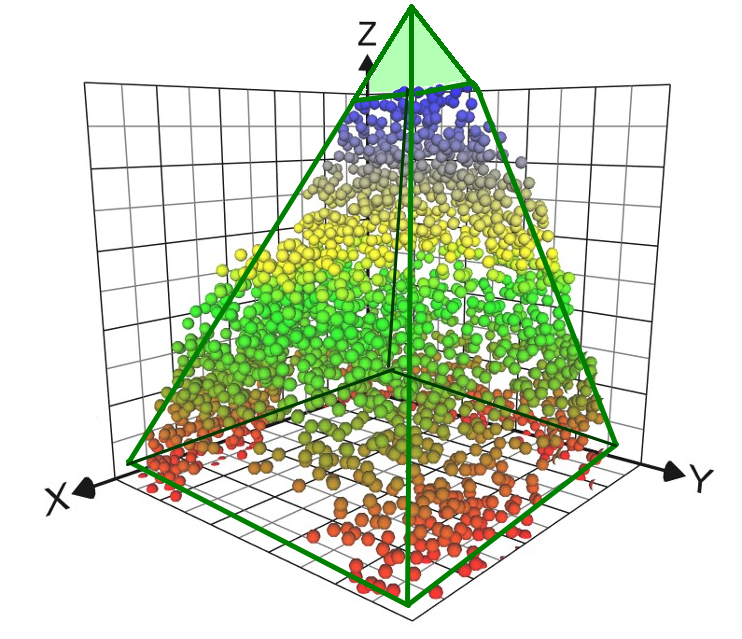
\includegraphics[width=\textwidth]{reconstruction2.png}
            \caption[] {{\small Reconstruction scenario 2 - extending planes to a point intersection}}    
            \label{fig:rec2}
        \end{subfigure}
        \caption[]{\small An example problem and solution} 
        \label{fig:example}
    \end{figure*}
    
    
    \end{document}
    